Es wurden die Gatterverzögerungszeiten verschiedener Schaltkreisfamilien
mithilfe der Delaymessung des Oszilloskops ermittelt, die Ergebnisse sind in
Tabelle \ref{tab:verzug} zu sehen.

\begin{table}[]
  \begin{center}
\begin{tabular}{c|c|c}
\rowcolor{gray0} 
Familie & \begin{tabular}[c]{@{}l@{}}Verzögerungszeit, \\ gemessen $/ \, \si{\nano\second}$\end{tabular} & \begin{tabular}[c]{@{}l@{}}Verzögerungszeit, \\ Datenblatt (SNx00, max. Werte) $/ \, \si{\nano\second}$\end{tabular} \\
7400    & 56.3                                                                                           & 22                                                                                                                \\
74LS00  & 43.8                                                                                           & 15                                                                                                                \\
74ALS00 & 30.5                                                                                           & 15                                                                                                                \\
74HC    & 48.4                                                                                           & 23                                                                                                                \\
74HCT   & 46.9                                                                                           & 25                                                                                                                \\
74F00   & 18.1                                                                                           & 6                                                                                                                 \\
4011    & 570                                                                                            & 250                                                                                                              
\end{tabular}
\end{center}
\caption{Mess- und Datenblattwerte der Verzögerungszeit verschiedener Schaltkreisfamilien}
\label{tab:verzug}
\end{table}


Für jede Familie wurde dann der entsprechende Maximalwert des \textit{propagation delays}
($t_{\textrm{pd}} / t_\textrm{PLH}$) , wie er in den Datenblättern der
jeweiligen Familie (für Hersteller \textsc{Texas Instruments},
jeweils NAND Gatter) angegeben ist, zum Vergleich herausgesucht. 
Dies sind nur Schätzwerte, da die genauen Testbedingungen nicht bekannt sind, es
zeigt jedoch signifikante Abweichungen der gemessenen und in den Datenblättern
angegebenen Werte, welche möglicherweise auf die Alterung der Schaltkreise
zurückzuführen sind, die Beziehungen der Schaltkreisfamilien untereinander bleiben
jedoch annäherungsweise bestehen.

  \begin{figure}[h]
  \begin{center}
    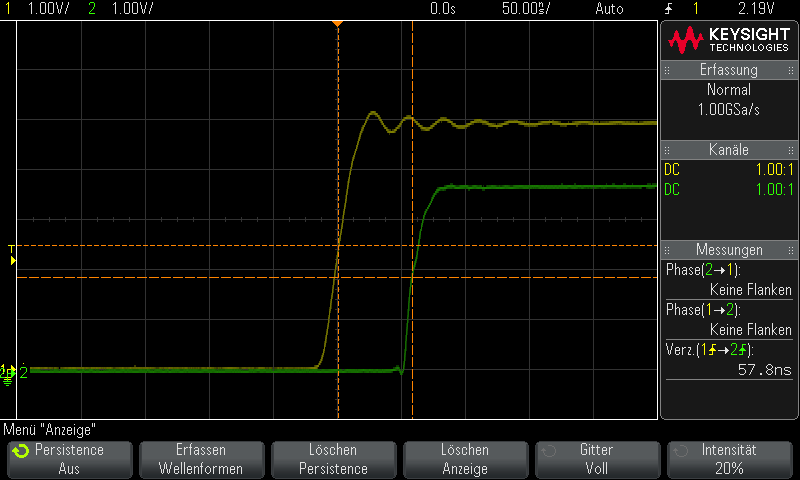
\includegraphics[width=\textwidth]{VERA/Verzoegerungszeit/74000}
  \end{center}
  \caption{Messung der Verzögerungszeit am Oszilloskop (7400)}
  \label{fig:biepbiep}
\end{figure}
